\documentclass[12pt]{article} 
\usepackage{graphicx} % Required for inserting images
\usepackage{amsmath}
\usepackage{subcaption} 
\usepackage[scale=0.8]{geometry}
\usepackage{cite}

\title{Investigating unconventional superconductivity in the 2D Hubbard-Kanamori model using Functional Renomarlization Group (FRG)}
\author{210003218}
\date{February-May 2025}

\begin{document}
\maketitle
\tableofcontents 


\section{Abstract}

\section{Introduction}

\section{Theoretical Background}

\subsection{Unconventional superconductivity}

\subsubsection{Spin-fluctuation mediated superconductivity}

\subsection{Hubbard-Kanamori Model}

\subsubsection{Tight Binding Models}

The Tight Binding Model is a central element of condensed matter physics \eqref{TBM}. In this model, electrons are bound in orbitals (called sites) around the lattice ions.
Due to the overlap between the quantum mechanical wavefunctions that describe these sites, electrons are allowed to 'hop' to neighbouring sites. The probability that this hopping process will occur is given by a tunnelling amplitude, which can be calculated using a hopping integral. \par
\medskip
\noindent This work is carried out in the tight-binding model framework, where the magnitude of the tunnelling amplitudes are at first treated as free parameters. 
Here, we build from a simple 2D nearest neighbour hoppping Hubbard model (Section.~\ref{subsec: HubbardModel}) and investigate the effect of introducing and varying the strength of the next-nearest neighbour hopping amplitude (See Fig. \ref{fig:2D Hubbard model}).
We extend these models further by considering the two-orbital per site case. 



\begin{equation} \label{TBM}
    \hat{H}_{TB}(\b{R}) = \sum_{ij\sigma} t_{ij}(\hat{c}_{i\sigma}^{\dagger}\hat{c}_{j \sigma} + h.c)
\end{equation}


\begin{figure}[htbp]  % Placement: Here, Top, Bottom, Page
    \centering
    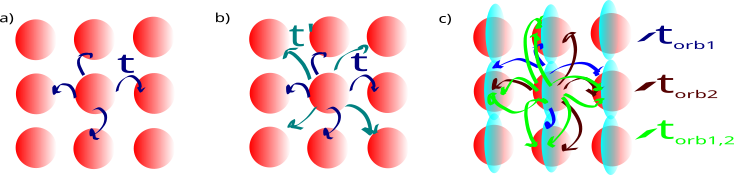
\includegraphics[width=0.9\textwidth]{2Dhubbardmodel.png}  % Adjust width as needed
    \caption{\textbf{Two-Dimensional Tight-Binding Models:} Three pannels showing the 1NN, 1NNN and 1NN2 models discussed in Section~\ref{subsec:1NNModel},~\ref{subsec:1NNNModel} and~\ref{subsec:1NN2Model} respectively. Fig a) shows the Nearest-neighbour hopping case, where \textit{t} depicts the hopping amplitude between the neighbouring sites. Fig b) shows the inclusion of the next-nearest neighbour hopping, the magnitude given by \textit{t'}.
    Fig c) Shows the extension to the two-orbital case, depicting the same orbital ($t_{orb1}$, $t_{orb2}$) and different orbital ($t_{orb1,2}$) nearest neighbour hopping. Note that this is just a pictorial representation of the orbitals, and that it does not correspond to a particular choice of orbitals or their real space projection. }
    \label{fig:2D Hubbard model}
\end{figure}

\newpage

\subsubsection{Hubbard Model}
\label{subsec: HubbardModel}

The  tight binding model as defined above fails to account for any interactions between neighbouring electrons. This motivates the extension of this model to the Hubbard model \eqref{t Hubbard model}, which includes the (onsite) Coulomb repulsion between electrons. Despite its simple form, this model can describe very rich physical phenomena.
In particular, it becomes very interesting to study when U and t are of comparable order, since it highlights the competing phenomena that takes place in correlated systems. 
The 2D Hubbard model remains unsolved to date, but is able to predict all sorts of correlated phases: it describes metals, insulators, superconductors and other exotic phases (REFERENCE). 
This model has been widely studied since it resembles the structure of the cuprate high-temperature superconductors (REFERENCE). While it has shown to accurately  capture the magnetic and superconducting behaviour that is expected of this family of superconductors, recent findings suggest that the superconducting groundstate 
could indeed be an artefact of some numerical approximation (REFERENCE-ABSENCE...). A large part of this thesis focuses on exploring this toy model and the effect of the nearest-neighbour hopping parameter.



\begin{equation}\label{t Hubbard model}
    \hat{H} = \sum_{ij\sigma} -t_{ij}(\hat{c}_{i\sigma}^{\dagger}\hat{c}_{j \sigma} + h.c) 
    + U \sum_{i} \hat{n}_{i \uparrow} \hat{n}_{i \downarrow}
\end{equation}





\subsubsection{Hubbard-Kanamori Model}
In the case of materials with a multi-band and/or multi-orbital nature, the Hubbard model is not sufficient to capture all of the physical phenomena. This motivates the extension of the Hubbard Model to the Hubbard- Kanamori model by including a Hund's coupling term.
Solving this Hamiltonian is rather challenging, which is why we resort to numerical techniques such as FRG to do so. 

\begin{equation} \label{Hubbard-Kanamori Model}
    H_{int} = U \sum_{is}n_{i,s\uparrow}n_{i,s\downarrow} + \frac{V}{2} \sum_{i,s,t \neq s} n_{is}n_{it} -\frac{J}{2} \sum_{i,s,t \neq s} \vec{S}_{is} \cdot \vec{S}_{it} 
    + \frac{J'}{2} \sum_{i,s,t \neq s} \sum_{\sigma} c_{is\sigma}^{\dagger}c_{is\bar{\sigma}}^{\dagger}c_{it\bar{\sigma}}c_{it\sigma}
\end{equation}

Here, $U$ and $V$ represent the intraorbital interaction of electrons in the same and different orbitals respectively. For generality, the intraorbital exchange $J$ and the 'pair hopping' term $J'$ following from Hund's rule coupling have been separated.  
Note that this Hamiltonian is relevant for the later section of this project, where the model is extended to a two-orbital, two-dimensional Hubbard Model.

\subsection{Theoretical Background in FRG}

\begin{figure}[htbp]  % Placement: Here, Top, Bottom, Page
    \centering
    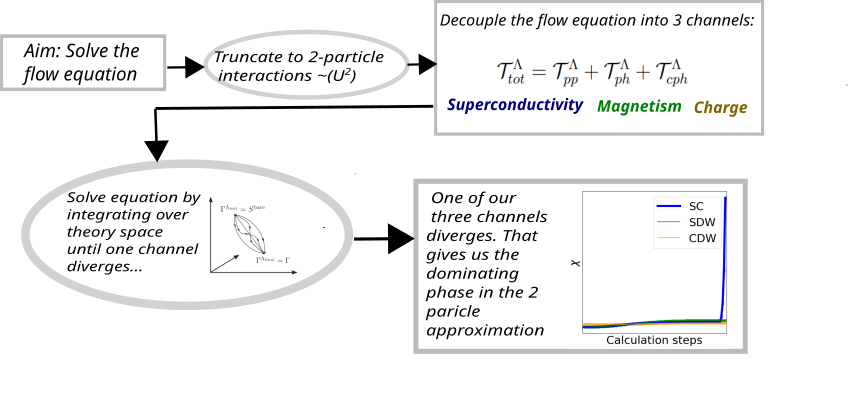
\includegraphics[width=0.9\textwidth]{FRGflowdiagram.png}  % Adjust width as needed
    \caption{\textbf{FRG Flowchart:} Schematic diagram outlining the TU$^2$FRG calculation steps. Starting from the flow equation and applying the truncation scheme in order to decouple the action into three "physical" terms. 
    The flow equation can then be solved by calculating each channel separatedly and taking the dominating phase to be the channel that diverges.}
    \label{fig:FRGflowdiagram}
\end{figure}

\subsubsection{Flow equation}

\subsubsection{Truncation scheme}

\subsubsection{Decoupling of flow equation}

\subsubsection{Instability calculation}



\section{Computational Methods}

\subsection{Diverge}

\subsection{Convergence of Calculation}

\subsubsection{Form factor convergence}

\subsubsection{Number of k points convergence }

\subsection{Calculation of Susceptibilities}

\subsubsection{Nesting vectors}

\subsubsection{Superconducting order parameters}

\section{Results and discussion}

\subsection{1NN Model}
\label{subsec:1NNModel}

\begin{figure}[htbp]  % Placement: Here, Top, Bottom, Page
    \centering
    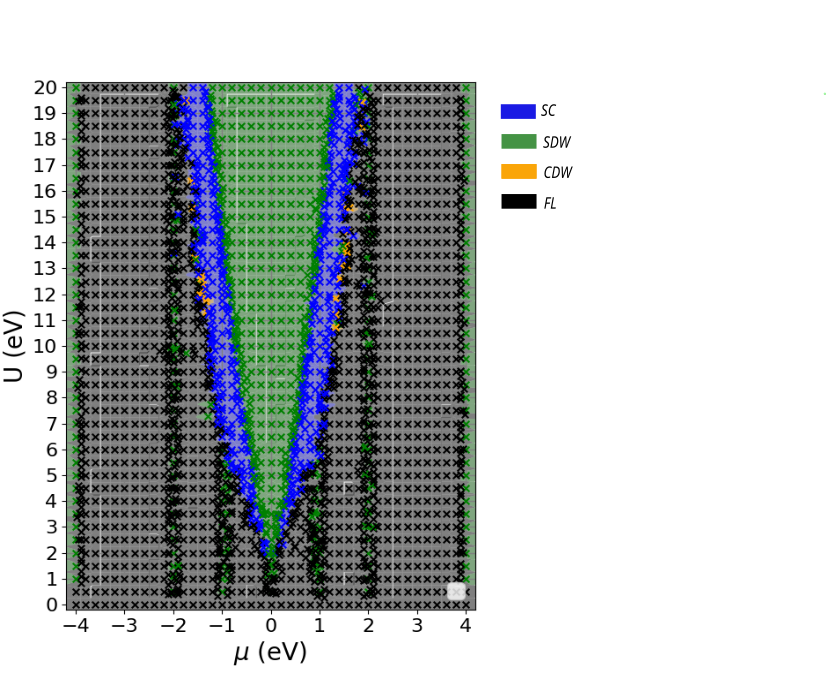
\includegraphics[width=1.25\textwidth]{1NNphasediagram.png}  % Adjust width as needed
    \caption{\textbf{Phase diagram for the 1NN model}:  (t =1eV, nkxnkf = 20x5, ff = 4\AA) as a function of On-site Coulumb Repulsion $U$ and chemical potential $\mu$. 
    Figure shows the four phases observed in the 1NN model: SC (Superconductivity), SDW (Spin-Density Wave), CDW(Charge Density Wave) and FL (Fermu-Liquid).
    Calculated points in the phase diagram are showed by the 'x' markers and a lighter-couloured background is used to depict interpolated regions between these points. }
    \label{fig:1NNpd}
\end{figure}


\subsubsection{Superconductivity in the 1NN Model}

\begin{figure}[htbp]  % Placement: Here, Top, Bottom, Page
    \centering
    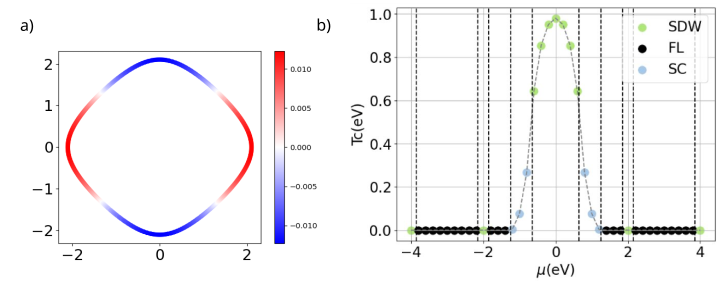
\includegraphics[width=1.0\textwidth]{1NNSC.png}  % Adjust width as needed
    \caption{\textbf{Superconductivity in the 1NN model}:  
    Fig a) Superconducting order parameter projected on Fermi Surface at $\mu$ = 1.00 eV, 
    for U =10.00eV. The order parameter is antisymmetric about a 90 degree rotation and hence
    it exhibits d-wave symmetry. 
    Fig b) Transition temperature (Tc) as a function of chemical potential ($\mu$) for U =10.00eV.
    Tc is enhanced closest to the magnetic instability.   
    }
    \label{fig:1NNSC}
\end{figure}



\subsubsection{Magnetic stripes in the 1NN Model}

\begin{figure}[htbp]  % Placement: Here, Top, Bottom, Page
    \centering
    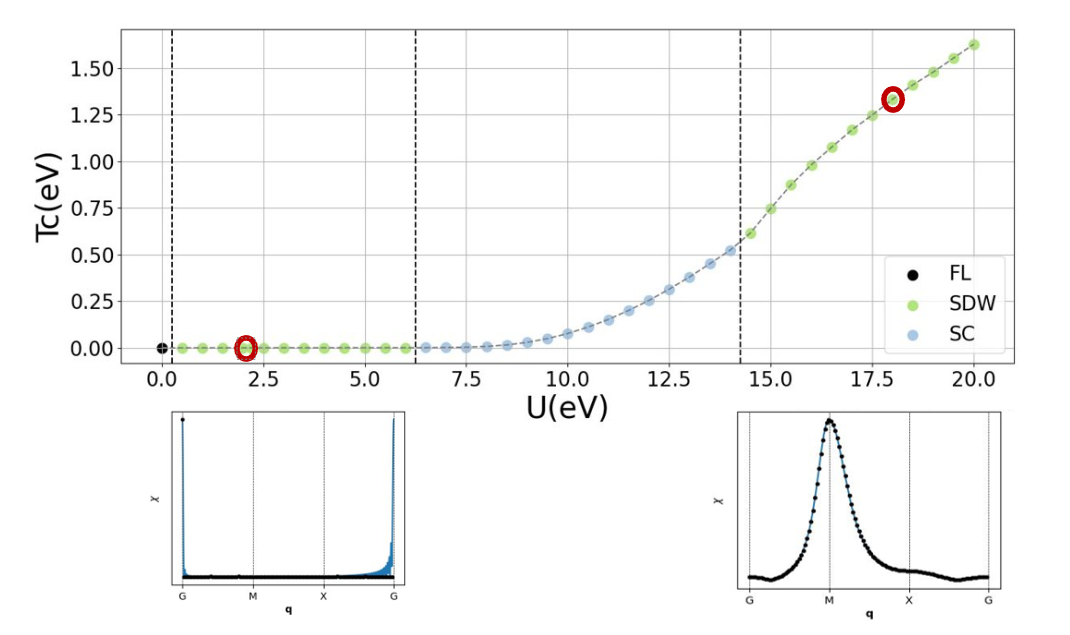
\includegraphics[width=0.9\textwidth]{1NN_SDW_stripes.png}  % Adjust width as needed
    \caption{Critical temperature as a function of Coulumb repulsion (U) along the Magnetic stripe at $\mu$ =1eV. Plots showing the susceptibility as a function of \b{q} for both magnetic regions. The Ferromagnetic SDW is supressed by a superconducting phase. At larger values of U, we recover the SDW phase but with an Anti-Ferromagnetic ordering instead.  }
    \label{fig:1NN_stripes}
\end{figure}


\subsection{Effect of next-nearest neighbour hopping (1NNN model)}
\label{subsec:1NNNModel}


\begin{figure}[htbp]  % Placement: Here, Top, Bottom, Page
    \centering
    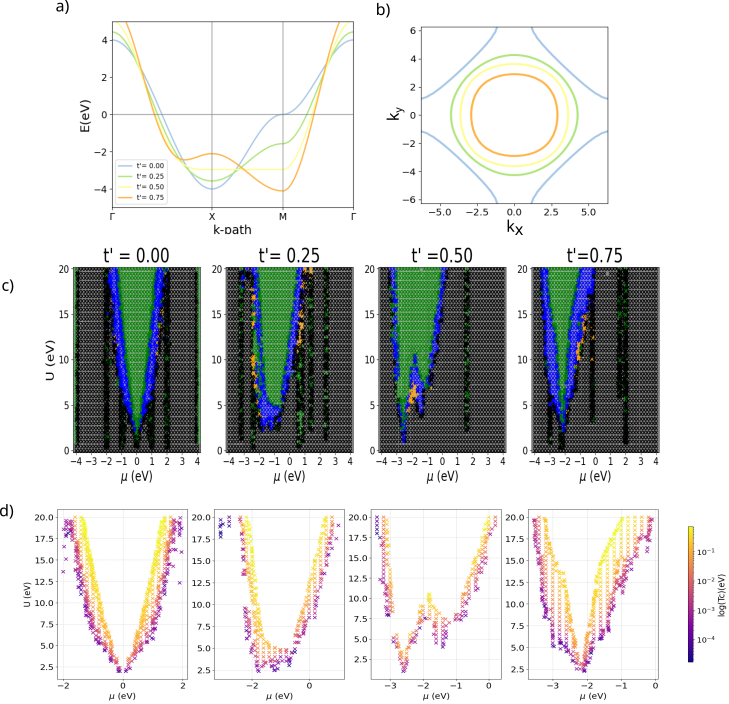
\includegraphics[width=1.0\textwidth]{1NNN.png}  % Adjust width as needed
    \caption{\textbf{1NNN model:} a) Phase diagram for the 1NNN model as a function of Coulumb repulsion U and chemical potential $\mu$ (t =1eV, nkxnkf = 20x5, ff = 4\AA) for t'=0.00, 0.25, 0.50, 0.75 eV. 
    b) Transition temperature for the superconducting region.
    c) Single plot of the band structure along high-symmetry path for corresponding values of t'.
    d) Single plot of the Fermi surface for all values of t' considered.}
    
    \label{fig:1NNN}
\end{figure}

\newpage

\subsubsection{Superconductivity in the 1NNN Model}



\subsubsection{Magnetic stripes in the 1NNN model}

\begin{table}[h]
    \centering
    \begin{tabular}{|c|c|c|c|c|c|c|}
        \hline
       t'(eV) & $\mu$ (eV) & Competing with other phase?& Nesting vector & Magnetic ordering  \\
        \hline
        0.00 & 1.00 & Yes (SC) & (0,0)-($\pi$, $\pi$)&  Changing from FM-AFM\\
        \hline
        0.00 & 2.00 &  No  & (0,0)-(0, $\pi$)  & Changing from FM to Commensurate\\
        \hline
        0.25 & 2.40 &  No  & (0,0)  & FM \\
        \hline
        0.25 & 1.40 &  Yes (CDW)  & (0,0)  & FM \\
        \hline
        0.25 & -2.00 & No  & (0,0)-($\pi$, $\pi$)  & FM - AFM\\
        \hline
        0.25 & 0.60 &  No  & (0,0)  & FM \\
          
        \hline
    \end{tabular}
    \caption{\textbf{Survey of stripes in the 1NNN model.} Table summarising the location and magnetic ordering of the Stripes.}
    \label{tab:StripesSummary}
\end{table}

\subsection{Effect of bi-orbital system (1NN2 model)}
\label{subsec:1NN2Model}

\begin{table}[h]
    \centering
    \begin{tabular}{|c|c|c|c|c|c|c|}
        \hline
       Model &$t^{[1,0,0]}_{3z^2-r^2}$  &$t^{[0,1,0]}_{3z^2-r^2}$  &  $t_{x^2 - y^2}$ &  $t^{[1,0,0]}_{x^2 - y^2 -3z^2-r^2} $ & $t^{[0,1,0]}_{x^2 - y^2 -3z^2-r^2} $ & $t_{\perp}$ \\
        \hline
        & -0.781 & -0.719  &  -0.375 & -0.402 & -0.310 & -2.50\\
        \hline
        1NN2MN & on &  on  & on  & off & off & off \\
        \hline
        1NN2MY & on &  on  & on  & on & on & off \\
          
        \hline
    \end{tabular}
    \caption{\textbf{Nearest neighbour hopping parameters for 2D  two-orbital Hubbard models.} First row shows the calculated hopping parameters, note that  $t_{\perp}$ corresponds to the intralayer hopping between the $d_{3z^2-r^2}$ orbitals. Other rows show which hopping parameters were included in each of the two models.}
    \label{tab:2D2orbparams }
\end{table}

\subsubsection{Superconductivity in the 1NN2 model}

\subsubsection{Effect of orbital hybridisation in the 1NN2 model}



\section{Conclusion and Outlook}


\newpage

\bibliographystyle{unsrt}  % Choose a style such as plain, alpha, abbrv, etc.
\bibliography{references}

\end{document}